\chapter{Arhitektura i dizajn sustava}
		
		\textbf{\textit{dio 1. revizije}}\\

		
		Arhitekturu sustava možemo podijeliti na tri podsustava:
		\begin{itemize}
			\item Web preglednik
			\item Web poslužitelj
			\item Baza podataka
		\end{itemize}
	
		
		%unos slike
		\begin{figure}[H]
			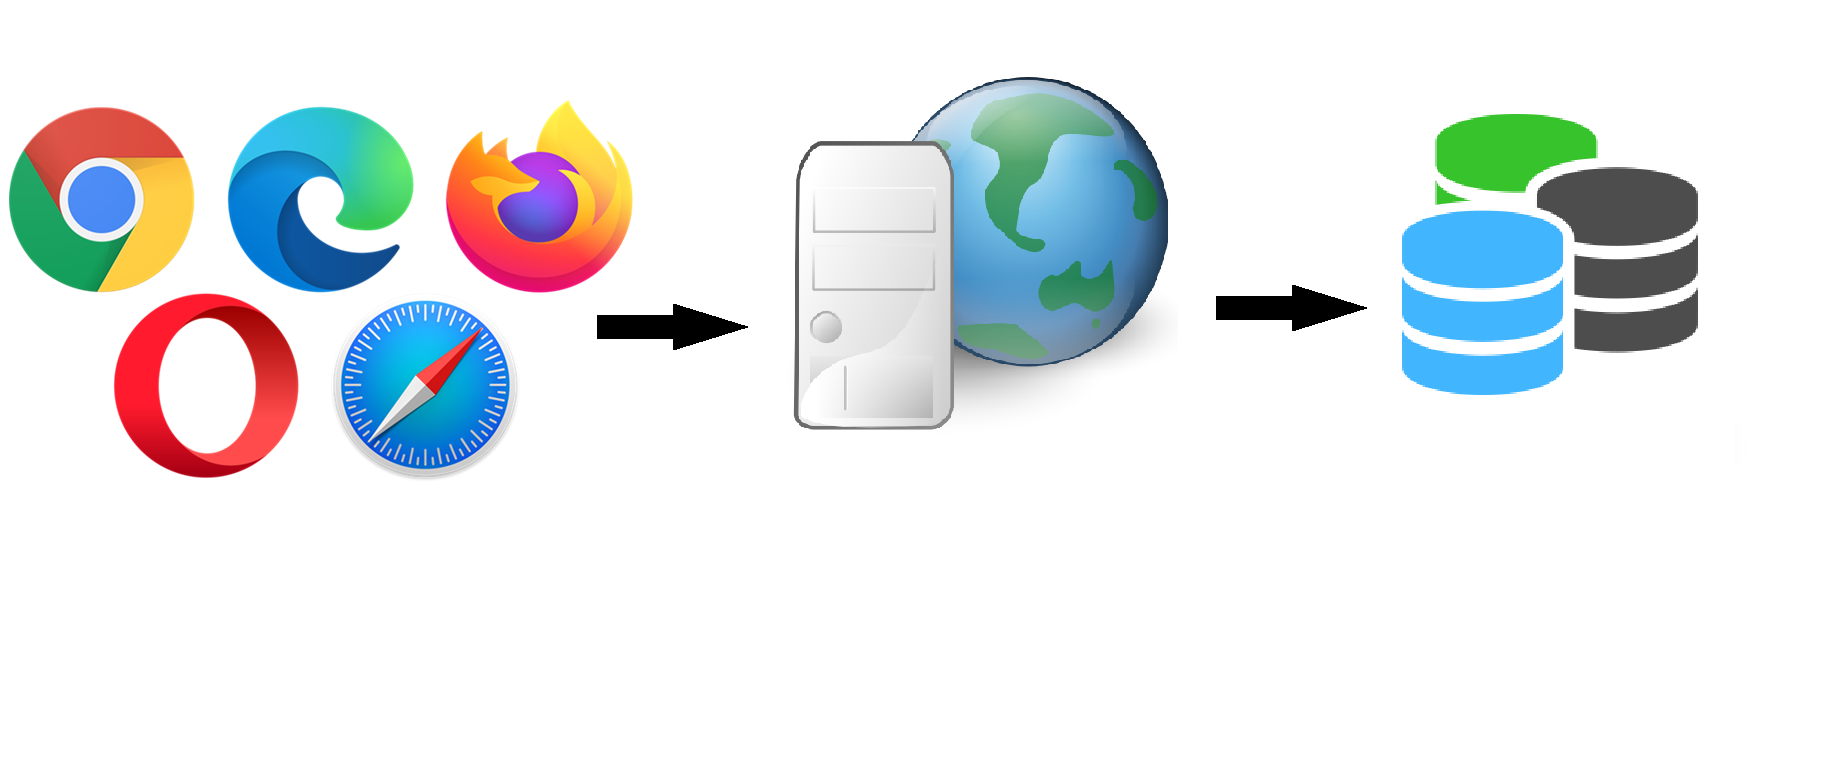
\includegraphics[scale=0.35]{slike/arhitektura.png} %veličina slike u odnosu na originalnu datoteku i pozicija slike
			\centering
			\caption {Arhitektura sustava}
			\label{fig:promjene}
		\end{figure}
		
		Korisnik pomoću web preglednika po vlastitom izboru dobiva mogućnost  pristupa web aplikaciji na  Internetu. Preglednik zapravo šalje zahtjev protokolom web poslužitelju na kojem se nalazi web aplikacija i on ju pokreteće i omogućuje korisniku daljnji rad na aplikaciji.
		
		Pred korisnikom se nalaze sve funkcionalnosti koje aplikacija pruža. On svojevoljno odabire pojedinu fukcionalnost te tako šalje zahtjev aplikaciji koja pristupa bazi podataka i prikuplja zatražene podatke i osvježava mu pregled aplikacije s prikupljenim podacima. 

		Sama aplikacija je sastavljena po načelu objektno usmjerene arhitekture. Razlog njezinog odabira je trenutna sveprisutnost u industriji te predstavlja standard razvoja složenih programskih zahtjeva. Budući da je razvoj aplikacije zamišljen kao rad više ljudi u timu  objektno usmjerena arhitektura nudi da se logički razdijeli sustav na više cjelina te time omogućuje paralelnost razvoja.
		Također nudi recikliranje koda, mogućnost dodavanja novih funkcionalnosti bez poteškoća i greške se lako detektiraju i ispravljaju.
		
		Aplikacija je razvijena u programskom jeziku Java 15 te kao razvojni okvir koristi Java Spring Boot verzije 2.3.4. Za sigurnost i spriječavanje vanjskih napada koristi se Spring Security.
		Kako bi se olakšala komunikacija s bazom koristi se Spring JDBC.  
		Za razvojno okruženje koristi se Ecplise i IntelliJ.
		 
		
		Frontend je pisan u  React. React je open-source, frontend, JavaScript knjižnica koja služi  za izgradnju korisničkog sučelja. Koristi HTML, CSS, JSX i JavaScript kako bi modelirao sučelje.
		
		Komunikacija između Jave na backendu i Reacta na frontendu je omogućena korištenjem REST api-ja.
			%unos slike
		\begin{figure}[H]
			
\includegraphics[scale=0.7]{slike/arhitektura2.jpg} %veličina slike u odnosu na originalnu datoteku i pozicija slike
			\centering
			\caption {Arhitektura sustava}
			\label{fig:promjene}
		\end{figure}
	
			\begin{figure}[H]
			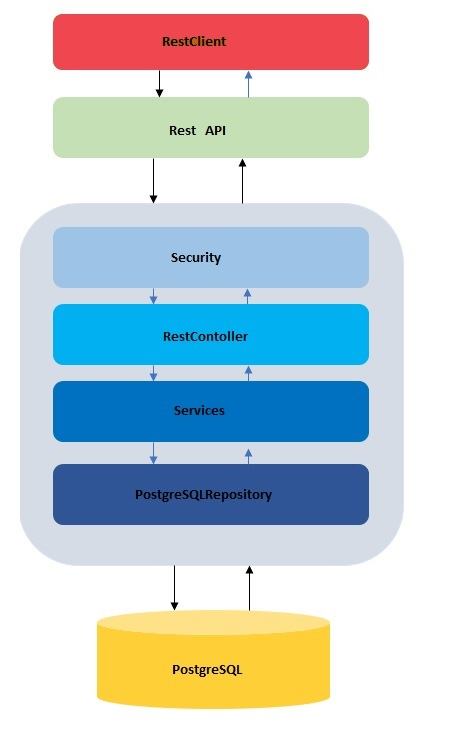
\includegraphics[scale=0.9]{slike/arhitektura3.jpg} %veličina slike u odnosu na originalnu datoteku i pozicija slike
			\centering
			\caption {Arhitektura sustava}
			\label{fig:promjene}
		\end{figure}

		\newpage	
		\section{Baza podataka}
			
			\textbf{\textit{dio 1. revizije}}\\
		
		Implementacija baze podataka ostvarena je uporabom PostgreSQL zbog jednostavnosti korištenja i pozitivnog iskustva članova tima. 
		
		Baza podataka sastoji se od sljedećih tablica:
		
		\begin{packed_item}
			\item Korisnik
			\item Zahtjev
			\item Lokacija
			\item Izvršavanje
			\item Kandidatura
			\item Kandidiranje
			\item Ocjenjivanje
			\item OcjenaIzvršavanja
			\item ImaUlogu 
			\item Uloga
			
		\end{packed_item}
		
			\subsection{Opis tablica}
			
					    \textbf{ Korisnik}
		    \text Ovaj entitet sadržava sve važne informacije o korisniku aplikacije. Sadrži atribute: ID${\_}$Korisnika, ime, prezime, email, lozinka, aktivan, token te duljinu i sirinu. Ovaj entitet je u vezi \emph{One-to-Many} s entitetom Zahtjev preko atributa ID${\_}$Korisnika,u vezi  \emph{One-to-Many} s Lokacijom prkeo atributa duljina i širina, u vezi s entitetom Kandidiranje preko atributa ID${\_}$Korisnika te u vezi \emph{One-to-Many} s entitetom Ocjenjivanje preko atributa ID${\_}$Korisnika gdje korisnik ima dvije uloge. 
				
				\begin{longtabu} to \textwidth {|X[6, l]|X[6, l]|X[20, l]|}
					
					\hline \multicolumn{3}{|c|}{\textbf{Korisnik}}	 \\[3pt] \hline
					\endfirsthead
					
					\hline \multicolumn{3}{|c|}{\textbf{Korisnik }}	 \\[3pt] \hline
					\endhead
					
					\hline 
					\endlastfoot
					
					\colorbox{LightGreen}{\textbf{ID${\_}$Korisnik}} & SERIAL	& jedinstveni identifikator korisnika 	 	\\ \hline
					ime & VARCHAR	&  ime korisnika	\\ \hline 
					prezime & VARCHAR	& prezime korisnika 		\\ \hline
					email & VARCHAR & e-mail adresa korisnika  \\ \hline 
					lozinka	& VARCHAR & hash lozinke 	\\ \hline  
					aktivan & BOOLEAN & status korisnika \\ \hline
					token & VARCHAR & JWT refresh token koji se koristi pri autentifikaciji korisnika \\ \hline
					 \colorbox{LightBlue}{\underline{ duljina} }& NUMERIC & geografska duljina \\ \hline
					 \colorbox{LightBlue}{\underline{ sirina}}	& NUMERIC & geografska širina  \\ \hline 
					
					
				\end{longtabu}
				    \textbf{ Zahtjev}
			    \text Ovaj entitet sadržava sve važne informacije o korisnikovu zahtjevu. Sadrži atribute: ID${\_}$Zahtjev, opis, datum, vrijeme, status, brojMobitela, ID${\_}$Autor, ID${\_}$Izvršitelj, duljina i sirina. Ovaj entitet je u vezi \emph{Many-to-one} s entitom Lokacija preko atributa sirina i duljina,također u vezi \emph{One-to-One} s entitetom Izvrsavanje preko atributa ID${\_}$Zahtjev te u dvije veze \emph{Many-to-One} s entitetom Korisnik preko ID${\_}$Korisnika što rezultira pojavom atributa ID${\_}$Autor i ID${\_}$Izvršitelj u tablici Zahtjev.  
			
				\begin{longtabu} to \textwidth {|X[6, l]|X[6, l]|X[20, l]|}
					
					\hline \multicolumn{3}{|c|}{\textbf{Zahtjev}}	 \\[3pt] \hline
					\endfirsthead
					
					\hline \multicolumn{3}{|c|}{\textbf{Zahtjev }}	 \\[3pt] \hline
					\endhead
					
					\hline 
					\endlastfoot
					
					\colorbox{LightGreen}{\textbf{ID${\_}$Zahtjev}} & SERIAL	&  jedinstveni identifikator zahtjeva	 	\\ \hline
					opis & VARCHAR	& opis zahtjeva 		\\ \hline 
					datum & DATE	& datum do kada se treba izvršiti zahtjev  		\\ \hline
					vrijeme & TIME & vrijeme do kada se treba izvršiti zahtjev \\ \hline 
					status	& VARCHAR & status zahtjeva  	\\ \hline
					brojMobitela & VARCHAR & broj mobitela autora zahtjeva? \\ \hline
					\colorbox{LightBlue}{\underline{ID${\_}$Autora}} & SERIAL & jedinstveni identifikator korisnika(autora zahtjeva) \\ \hline
					\colorbox{LightBlue}{\underline{ID${\_}$Izvršitelj}} & SERIAL & jedinstveni identifikator korisnika(izvršitelja zahtjeva) \\ \hline
					\colorbox{LightBlue}{\underline{duljina}} & NUMERIC & geografska duljina \\ \hline
					\colorbox{LightBlue}{\underline{ sirina}} & NUMERIC & geografsk širina    	\\ \hline 
					
				
				\end{longtabu}
			
			    \newpage
						    \textbf{ Lokacija}
			    \text Ovaj entitet sadržava sve važne informacije o lokaciji. Sadrži atribute: duljina i sirina,drzava, naselje te adresa.Ovaj entitet je u vezi \emph{One-to-many} s entitom Zahtjev preko atributa sirina i duljina, također u vezi \emph{Many-to-one}s entitetom Korisnikom preko atributa duljina i sirina te u vezi \emph{One-to-Many} s entitetom Kandidatura preko atributa duljina i sirina. 
			
				\begin{longtabu} to \textwidth {|X[6, l]|X[6, l]|X[20, l]|}
					
					\hline \multicolumn{3}{|c|}{\textbf{Lokacija}}	 \\[3pt] \hline
					\endfirsthead
					
					\hline \multicolumn{3}{|c|}{\textbf{Lokacija }}	 \\[3pt] \hline
					\endhead
					
					\hline 
					\endlastfoot
					
					\colorbox{LightGreen}{\textbf{duljina}} & NUMERIC	& geografska dužina \\ \hline
					\colorbox{LightGreen}{\textbf{sirina}} & NUMERIC & geografska sirina \\ \hline
					drzava & VARCHAR	& naziv države 		\\ \hline
					naselje & VARCHAR & naziv naselja  \\ \hline 
					adresa	& VARCHAR & adresa na kojoj treba odraditi zahtjev	\\ \hline 	
					
				\end{longtabu}
			
			
		    \textbf{ Izvršavanje}
		    \text Ovaj entitet sadržava sve važne informacije o izvršiteljima zahtjeva i podacima koji im omogućavaju samo izvršavanje. Sadrži atribute: ID${\_}$Zahtjev koji izvršavaju,  primljenNotif kao status o primitku notifikacije od strane korisnika. Ovaj entitet je u vezi \emph{One-to-many} sa Ocjenjivanje preko atributa ID${\_}$Zahtjev  i u vezi \emph{One-to-One} sa entitetom Zahtjev preko atributa ID${\_}$Zahtjev.

				\begin{longtabu} to \textwidth {|X[6, l]|X[4, l]|X[20, l]|}
					
					\hline \multicolumn{3}{|c|}{\textbf{Izvršavanje}}	 \\[3pt] \hline
					\endfirsthead
					
					\hline \multicolumn{3}{|c|}{\textbf{Izvršavanje}}	 \\[3pt] \hline
					\endhead
					
					\hline 
					\endlastfoot
					
					\colorbox{LightGreen}{\textbf{ID${\_}$Zahtjev}} & INT	& jedinstveni identifikator  \\ \hline
					primljenNotif & BOOLEAN & status o primitku notifikacije od strane korisnika  \\ \hline
				
					
					
				\end{longtabu}
			\textbf{ Kandidatura}
		    \text Ovaj entitet sadržava sve važne informacije o kandidaturi za korisnika godine. Sadrži atribute: godina kandidature, duljina i sirina. Ovaj entitet je u vezi \emph{Many-to-One} sa entitetom Kandidiranje preko atributa godina kandidature, geografska duljina i širina i u vezi \emph{Many-to-One} sa Lokacijom preko atributa duljina i sirina.

				\begin{longtabu} to \textwidth {|X[7, l]|X[6, l]|X[20, l]|}
					
					\hline \multicolumn{3}{|c|}{\textbf{Kandidatura}}	 \\[3pt] \hline
					\endfirsthead
					
					\hline \multicolumn{3}{|c|}{\textbf{Kandidatura}}	 \\[3pt] \hline
					\endhead
					
					\hline 
					\endlastfoot
					
					\colorbox{LightGreen}{\textbf{\underline{duljina}}} & NUMERIC	& geografska duljina  \\ \hline
					\colorbox{LightGreen}{\textbf{\underline{sirina}}} & NUMERIC	& geografska sirina  \\ \hline
					\colorbox{LightGreen}{\textbf{godina}} & INT & godina kandidature  \\[3pt] \hline 
				
					
				\end{longtabu}
				\newpage
				\textbf{Kandidiranje}
		    \text Ovaj entitet sadržava sve važne informacije o korisniku koji se kandidira za korisnika godine. Sadrži atribute: ID korisnika, godina, duljina i sirina. Ovaj entitet je u vezi \emph{One-to-Many} sa entitetom Kandidatura preko atributa godina kandidature, geografska duljina i širina te u vezi \emph{One-to-One} sa entitetom Korisnik preko atributa ID Korisnika.
		    
		    
		    	\begin{longtabu} to \textwidth {|X[7, l]|X[6, l]|X[20, l]|}
		    		
		    		\hline \multicolumn{3}{|c|}{\textbf{Kandidiranje}}	 \\[3pt] \hline
		    		\endfirsthead
		    		
		    		\hline \multicolumn{3}{|c|}{\textbf{Kandidiranje}}	 \\[3pt] \hline
		    		\endhead
		    		
		    		\hline 
		    		\endlastfoot
		    		\colorbox{LightGreen}{\textbf{\underline{ID${\_}$Korisnik}}} & SERIAL	& jedinstveni identifikator korisnika 	 	\\ \hline
		    		\colorbox{LightGreen}{\textbf{\underline{duljina}}} & NUMERIC	& geografska duljina  \\ \hline
		    		\colorbox{LightGreen}{\textbf{\underline{sirina}}} & NUMERIC	& geografska sirina  \\ \hline
		    		\colorbox{LightGreen}{\textbf{\underline{godina}}} & INT & godina kandidature  \\[3pt] \hline 
		    		
		    		
		    	\end{longtabu}
		    
		    
		    
		        \textbf{Ocjenjivanje}
		    \text Ovaj entitet sadržava sve važne informacije o međusobnom ocjenjivanju korisnika. Sadrži atribute:ID${\_}$Ocjenjivanje, {ID${\_}$Ocjenjeni korisnik te ID${\_}$Ocjenjivac, ocjena i komentar. Ovaj entitet je u dvostrukoj vezi \emph{Many-to-One} sa entitetom Korisnik preko atributa ID${\_}$Ocjenjeni i ID${\_}$Ocjenjivac te u vezi \emph{One-to-One} s entitetom Zahtjev preko atributa ID${\_}$Zahtjev.
		    
				\begin{longtabu} to \textwidth {|X[7, l]|X[6, l]|X[20, l]|}
					
					\hline \multicolumn{3}{|c|}{\textbf{Ocjenjivanje}}	 \\[3pt] \hline
					\endfirsthead
					
					\hline \multicolumn{3}{|c|}{\textbf{Ocjenjivanje }}	 \\[3pt] \hline
					\endhead
					
					\hline 
					\endlastfoot
					
					\colorbox{LightGreen}{\textbf{ID${\_}$Ocjenjivanje}} & INT	& jedinstveni identifikator ocjenjivanja 	\\ \hline
					ocjena & INT	&  ocjena usluge		\\ \hline 
					komentar & VARCHAR	& komentar ocjenitelja 		\\ \hline
					\colorbox{LightBlue}{\underline{ID${\_}$Zahtjev}} & SERIAL	&  jedinstveni identifikator zahtjeva	 	\\ \hline
					\colorbox{LightBlue}{\underline{ID${\_}$Ocjenjivac}} & INT	& jedinstveni identifikator ocjenjivaca 	\\ \hline
					\colorbox{LightBlue}{\underline{ID${\_}$Ocjenjeni}} & INT	& jedinstveni identifikator ocjenjenog 	\\ \hline
					
				\end{longtabu}
			
			
		
			\textbf{Uloga}
			\text Entitet sadržavi informaciju o ulozi korisnika tijekom korištenja aplikacije. Uloga može biti administrator ili obični korisnik. Sadrži atribute: ID${\_}$Uloga i naziv. U vezi \emph{Many-to-One} sa entitetom ImaUlogu preko atributa ID${\_}$Uloga.
			
			\begin{longtabu} to \textwidth {|X[6, l]|X[6, l]|X[20, l]|}
				
				\hline \multicolumn{3}{|c|}{\textbf{Uloga}}	 \\[3pt] \hline
				\endfirsthead
				
				\hline \multicolumn{3}{|c|}{\textbf{Uloga }}	 \\[3pt] \hline
				\endhead
				
				\hline 
				\endlastfoot
				
				\colorbox{LightGreen}{\textbf{ID${\_}$Uloga}}& SERIAL	&  jedinstveni identifikator uloge	 	\\ \hline
				naziv & VARCHAR	& naziv uloge 	\\ \hline
				
				
			\end{longtabu}
			\newpage
			\textbf{ImaUlogu}
			\text je vezna tablica koja sadržava informacije koji korisnik ima koju ulogu unutar aplikaicje.Sadrži atribute:ID${\_}$Korisnik i ID${\_}$Uloga. U vezi je \emph{One-to-Many} sa entitetom Uloga preko atributa ID${\_}$Uloga te u vezi \emph{One-to-Many} sa entitetom Korisnik preko atributa ID${\_}$Korisnik.
			
			\begin{longtabu} to \textwidth {|X[6, l]|X[6, l]|X[20, l]|}
				
				\hline \multicolumn{3}{|c|}{\textbf{ImaUlogu}}	 \\[3pt] \hline
				\endfirsthead
				
				\hline \multicolumn{3}{|c|}{\textbf{ImaUlogu }}	 \\[3pt] \hline
				\endhead
				
				\hline 
				\endlastfoot
				\colorbox{LightGreen}{\textbf{ID${\_}$Korisnik}} & SERIAL	& jedinstveni identifikator korisnika 	 	\\ \hline
				\colorbox{LightGreen}{\textbf{ID${\_}$Uloga}} & SERIAL	&  jedinstveni identifikator uloge	 	\\ \hline
				
				
				
			\end{longtabu}
		
		   \newpage
			\subsection{Dijagram baze podataka}
			
			
			%unos slike
			\begin{figure}[H]
				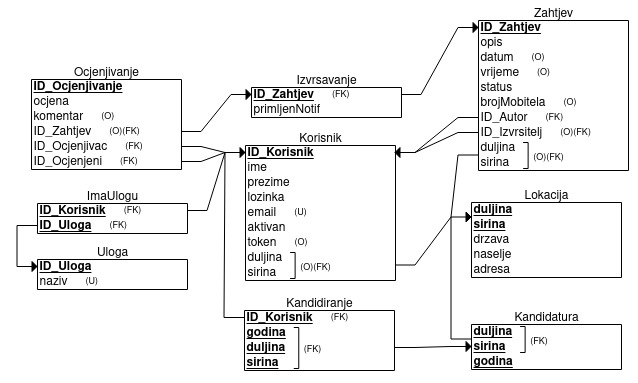
\includegraphics[scale=0.77]{slike/baza_podatakaNEW.jpeg} %veličina slike u odnosu na originalnu datoteku i pozicija slike
				\centering
				\caption {Dijagram baze podataka}
				\label{fig:promjene}
			\end{figure}
			
			\eject
			
		\section{Dijagram razreda}
		
			\textit Na slikama 4.5, 4.6, 4.7, 4.8 i 4.9 su prikazani dijagrami razreda za backend. Raspoređeni su u više slika radi bolje preglednosti i slične funkcionalnosti. Iz samih slika lakše se može uočiti povezanost samih stavki, njihova ovisnost te sadržaj atributa i funkcionalnosti.
			%unos slike
			\begin{figure}[H]
				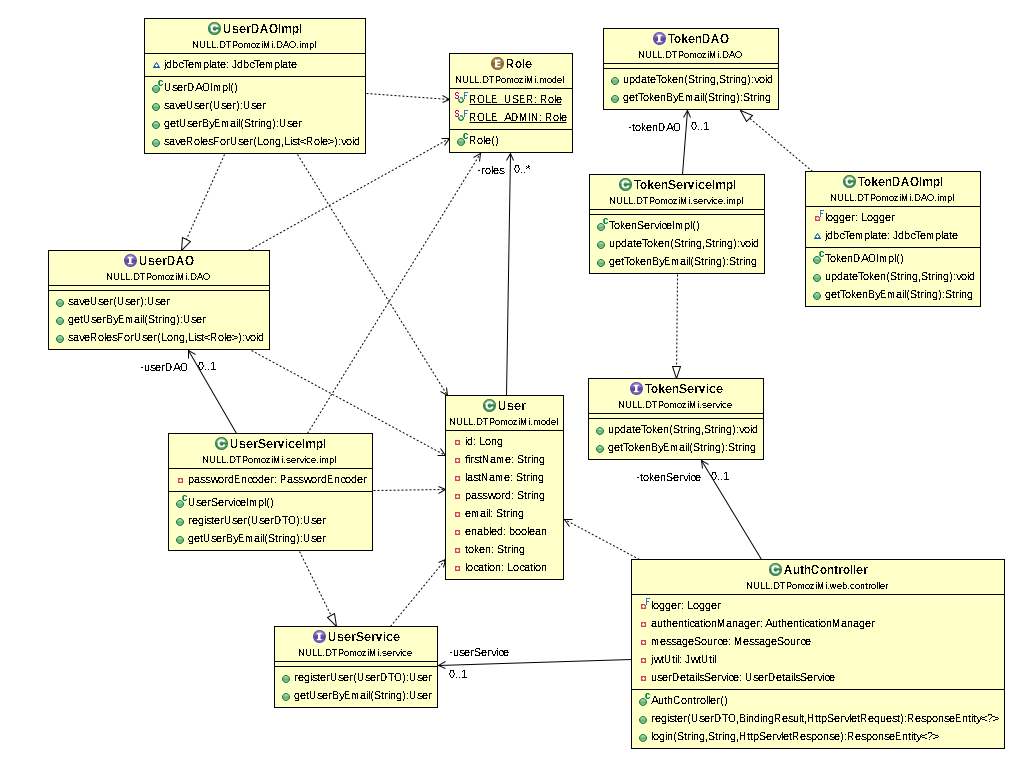
\includegraphics[scale=0.65]{slike/user.png} %veličina slike u odnosu na originalnu datoteku i pozicija slike
				\centering
				\caption { Dijagram razreda za User}
				\label{fig:promjene}
			\end{figure}
		
			%unos slike
			\begin{figure}[H]
				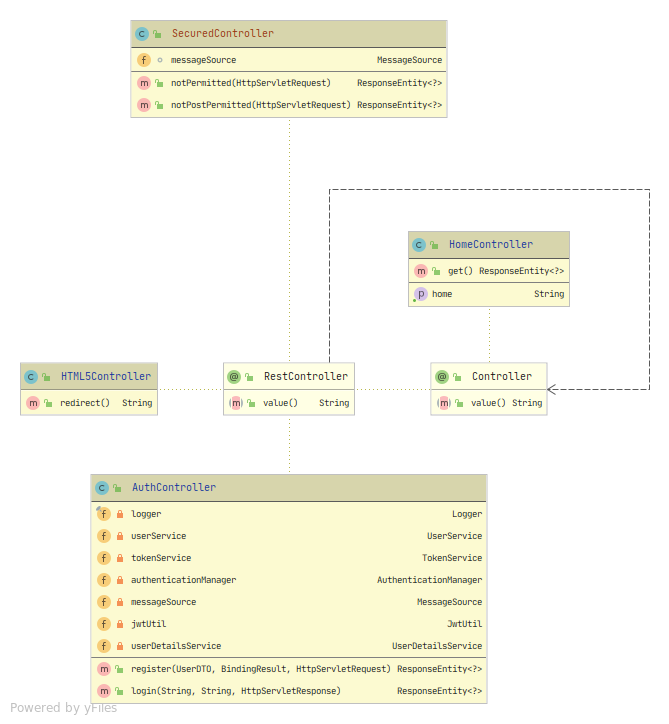
\includegraphics[scale=0.65]{slike/ControllersDiagram.png} %veličina slike u odnosu na originalnu datoteku i pozicija slike
				\centering
				\caption { Dijagram razreda za controllere}
				\label{fig:promjene}
			\end{figure}
			
			%unos slike
			\begin{figure}[H]
				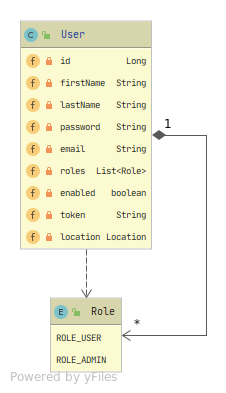
\includegraphics[scale=0.65]{slike/ModelUml.png} %veličina slike u odnosu na originalnu datoteku i pozicija slike
				\centering
				\caption { Dijagram razreda za model korisnika}
				\label{fig:promjene}
			\end{figure}
			
			
			%unos slike
			\begin{figure}[H]
				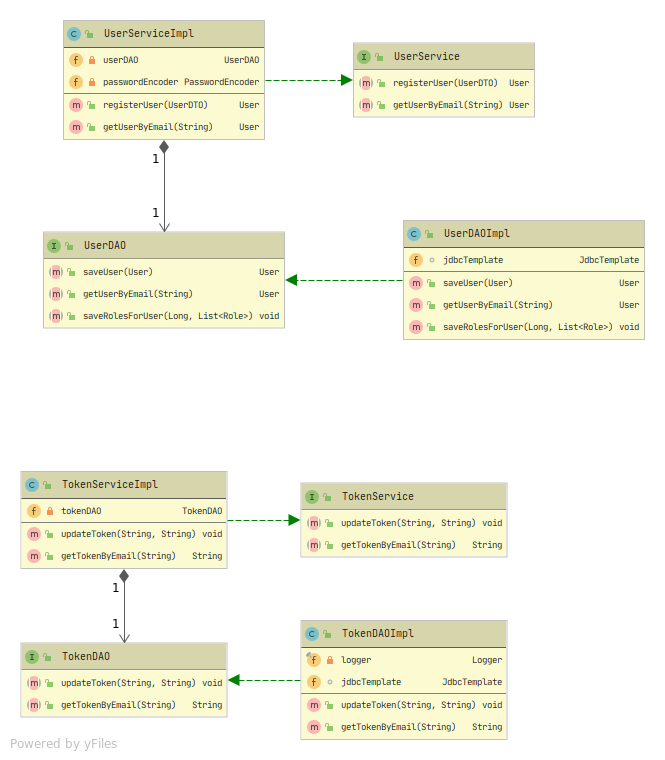
\includegraphics[scale=0.65]{slike/ServiceDaoUml.png} %veličina slike u odnosu na originalnu datoteku i pozicija slike
				\centering
				\caption { Dijagram razreda za ServiceDao}
				\label{fig:promjene}
			\end{figure}
			
			
			%unos slike
			\begin{figure}[H]
				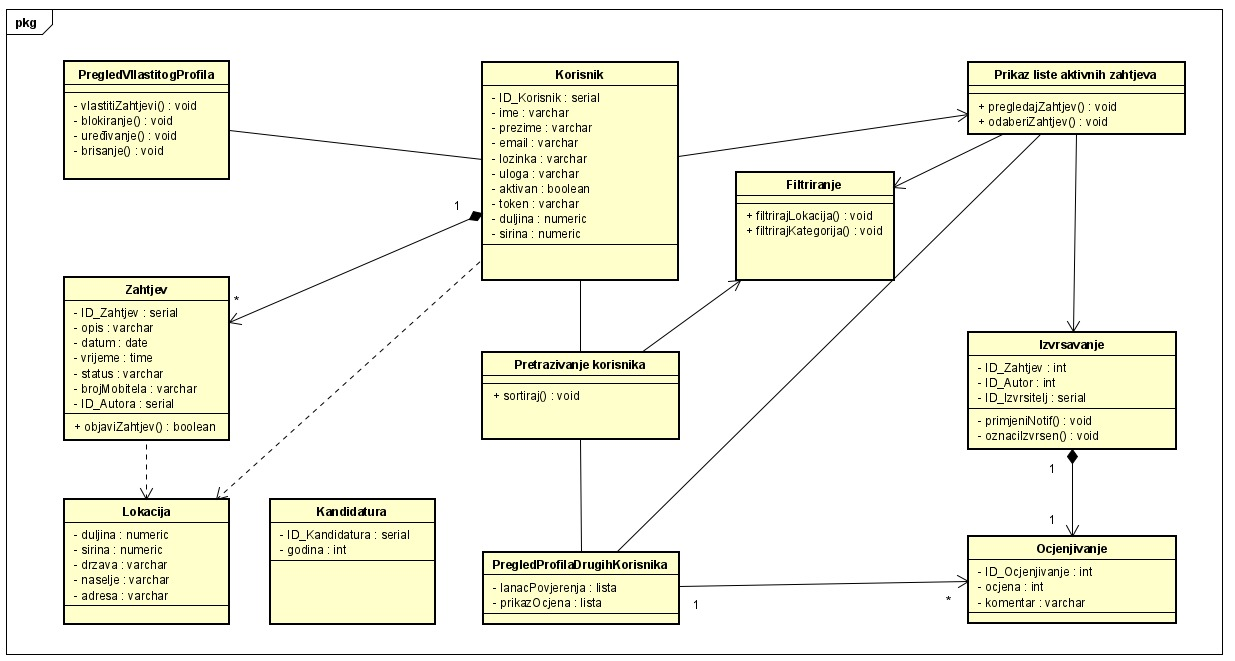
\includegraphics[scale=0.4]{slike/class_dijagram.jpeg} %veličina slike u odnosu na originalnu datoteku i pozicija slike
				\centering
				\caption { Dijagram razreda - models}
				\label{fig:promjene}
			\end{figure}

			\begin{comment}
			
			\textbf{\textit{dio 2. revizije}}\\
			
			
			\begin{comment}
			\textbf{\textit{dio 2. revizije}}\\			
			
			\textit{Prilikom druge predaje projekta dijagram razreda i opisi moraju odgovarati stvarnom stanju implementacije}
			\end{comment}
			
			
			
\begin{comment}		
		\section{Dijagram stanja}
			
			
			\textbf{\textit{dio 2. revizije}}\\
			
			\textit{Potrebno je priložiti dijagram stanja i opisati ga. Dovoljan je jedan dijagram stanja koji prikazuje \textbf{značajan dio funkcionalnosti} sustava. Na primjer, stanja korisničkog sučelja i tijek korištenja neke ključne funkcionalnosti jesu značajan dio sustava, a registracija i prijava nisu. }
			
			
			\eject 
		
		\section{Dijagram aktivnosti}
			
			\textbf{\textit{dio 2. revizije}}\\
			
			 \textit{Potrebno je priložiti dijagram aktivnosti s pripadajućim opisom. Dijagram aktivnosti treba prikazivati značajan dio sustava.}
			
			\eject
		\section{Dijagram komponenti}
		
			\textbf{\textit{dio 2. revizije}}\\
		
			 \textit{Potrebno je priložiti dijagram komponenti s pripadajućim opisom. Dijagram komponenti treba prikazivati strukturu cijele aplikacije.}
\end{comment}